\documentclass[aps, preprint]{revtex4-2}

\usepackage{graphicx}
\usepackage{amsmath}
\usepackage{amssymb}
\usepackage{hyperref}
\usepackage{xcolor}

\begin{document}

\title{Some model tests}

\author{Author Name}
\affiliation{Affiliation}

\date{\today}

\begin{abstract}
Some numerical tests about training and testing of cross section fitting 
using neural networks
\end{abstract}

\maketitle

\section{Introduction}
\label{sec:intro}

We use a neural network as universal interpolator to 
fit calculations of total cross sections (TCS) using two theoretical 
models, namely the Continuum-Distorted-Wave with Eikonal-Initial
-State (CDW-EIS) and the Classical Trajectory MonteCarlo (CTMC)
for ionization of hydrogen by bare ion impact. Here we consider
bare projectiles with charges $Z_P$ ranging between 1 and 9 

\section{Methods}
\label{sec:methods}

\subsection{The training set}
The training set consist of a number of $1013$ TCS. We have 
calculated $ 513 $ TCS with the CDW-EIS model and the CTMC model 
as it is specified in Table \ref{Table-TS}. It is important to 
note that we have considered here the semiempirical-model of Rudd 
(RSEM) [poner cita] on an equal footing with the theoretical models.

\begin{table}[h!]
\centering
\begin{tabular}{|c|c|c|c|}
\hline
\textbf{Theory} & Number of Impact Energies & 
Impact Energy Range (keV/amu) & Ion charges\\ \hline
\textbf{CDW-EIS} & 37 & 10 - 100000 & 1 - 9\\ \hline
\textbf{CTMC} & 20 & 15 - 2500 & 1 - 9\\ \hline
\textbf{Semi Empiric} & 500 & 10 - 5000 & 1\\ \hline

\end{tabular}
\caption{Number and energy range of TCS calculated for each model.}
\label{Table-TS}
\end{table}

The input variables are, the impact energy,
the projectile charge, and the theory used to obtain the TCS.
Since MLPs are not suitable for handling very tiny numbers nor 
several orders of magnitude, as in the case of this 
training set, we must perform a preprocessing stage that 
includes data compression by taking the decimal logarithm of the 
impact energy and the TCS. This preprocessing allow us to 
avoid gradient vanishing in the backpropagation algorithm 
used to fit the data due to the use of tiny floating point 
values for the energy and the TCS. Moreover, logarithm produce
a compression of the several orders of magnitude that TCS 
present for the wide impact energies considered here.  
On the other hand, the categorical 
variable corresponding 
to the theory must be cast to a numerical value. We choose 
to expand a three dimensional One Hot Encoding for the three 
theories considered here.

\subsection{The model}

We show in Figure \ref{fig:scheme} a scheme of the model used 
in this work. After the preprocessing stage we have a MLP with a 
5-dimensional input, then the hidden layers ($N_L$) and a single output 
corresponding to the $\log_{10}$ of the TCS.

\begin{figure}[htbp]

    \centering
    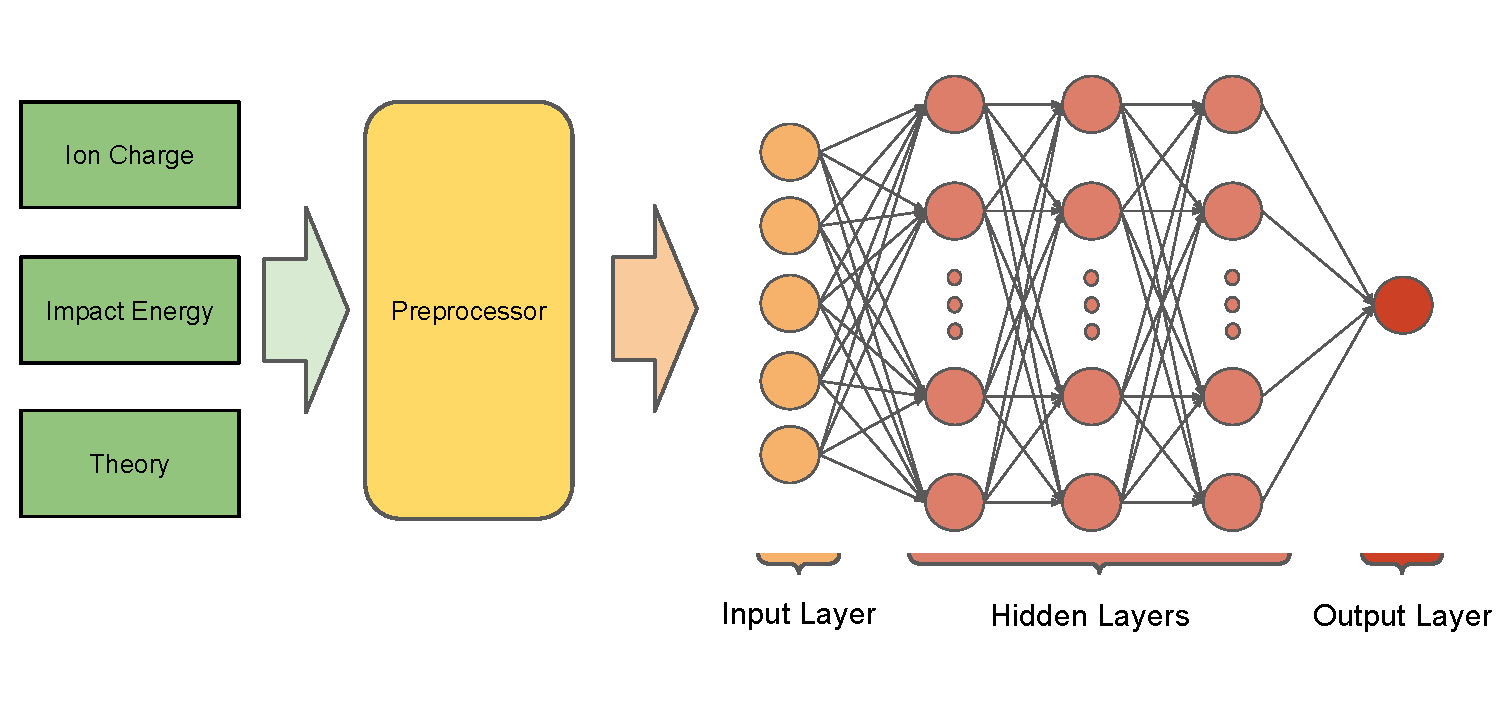
\includegraphics[width=0.8\textwidth]{./Esquema_ionNN.pdf}
    \caption{Interpolator scheme}
    \label{fig:scheme}
\end{figure}

To find the best architecture of the MLP, as the 
training set is not big enough, we have performed averaging
over a k-fold split over the training set, and the corresponding 
training for models with hidden layers ranging from one to five 
($N_L = 1,...5$), 
with different number of units per layer ($N_H = 2^n$ for $n = 
\{4,...,8\}$).
As it is well known, to introduce non linearity in the MLPs, 
non linear activation functions must be used for each unit 
output. Unlike the usual trend to use the fast-to-compute 
Rectifier Linear Unit activation function (ReLU), in this work we use 
two kinds of infinitely differentiable functions: the hyperbolic 
tangent, and a gaussian activation. The choice of smooth 
activation functions can be easily justified by the fact that 
TCS are smooth functions of the impact energy, and extreme 
non-differentiable oscillating fits caused by ReLU and its 
variations are naturally avoided.

This fitting process is a typical supervised learning. In supervised 
learning some \emph{distance} function between the model prediction $y_{pred}$ 
and the true value $y_{true}$ must be computed. This \emph{distance} 
function, is called the loss function $\mathcal{L}_{\theta}$, where $\theta$ 
refers to the MLP parameters. In this work we explore two loss functions

\begin{align}
    \mathcal{L}_{\theta}^{LCH}(y_{true},y_{pred}) & =  
    \log[\cosh(y_{pred} - y_{true})] \label{Eq-loss-lch}  \\
    \mathcal{L}_{\theta}^{ERR}(y_{true},y_{pred}) & =  
    L_1(y_{pred},y_{true}) + L_2(y_{pred},y_{true}) + Rel(y_{pred},y_{true}) 
    \label{Eq-loss-err}  
\end{align}    

In Eq. (\ref{Eq-loss-err}) three different metrics are added,
\begin{align}
    L_{1}(y_{true},y_{pred}) & =  \frac{1}{N} 
    \sum_{i=1}^{N}{ \left| y_{pred} - y_{true} \right|}
    \label{Eq-l1-mae}  \\
    L_{2}(y_{true},y_{pred}) & =  \frac{1}{N} 
    \sum_{i=1}^{N}{ \left( y_{pred} - y_{true} \right) ^2}
    \label{Eq-l2-mse}  \\  
    R(y_{true},y_{pred}) & =  \frac{1}{N} 
    \sum_{i=1}^{N}{ \left| \frac{y_{pred} - y_{true}}{y_{true}} \right|}.
    \label{Eq-rel-rel}
\end{align}

Usually, $L_1$, $L_2$, and $R$ are named as the mean 
absolute error (MAE), the mean squared error (MSE) and 
the mean relative error (MRE), respectively. We combine these three 
measures in order to guide the optimization algorithm 
for the different ranges in the $\log_{10}(TCS)$. 
While on one hand MSE emphasizes big differences, especially 
where target values are higher, the MAE does it at intermediate 
regions. On the other hand, $R$ runs over whole range 
on equal footing.

As we are dealing with analytic activation functions, 
we can use the gradient descent algorithm 
or any variant of it. In this work we use the Adam 
algorithm with an initial learning rate of $lr=1\times10^{-4}$
to \emph{backpropagate} the model and update the parameters.

\begin{figure}[htbp]
    \centering
    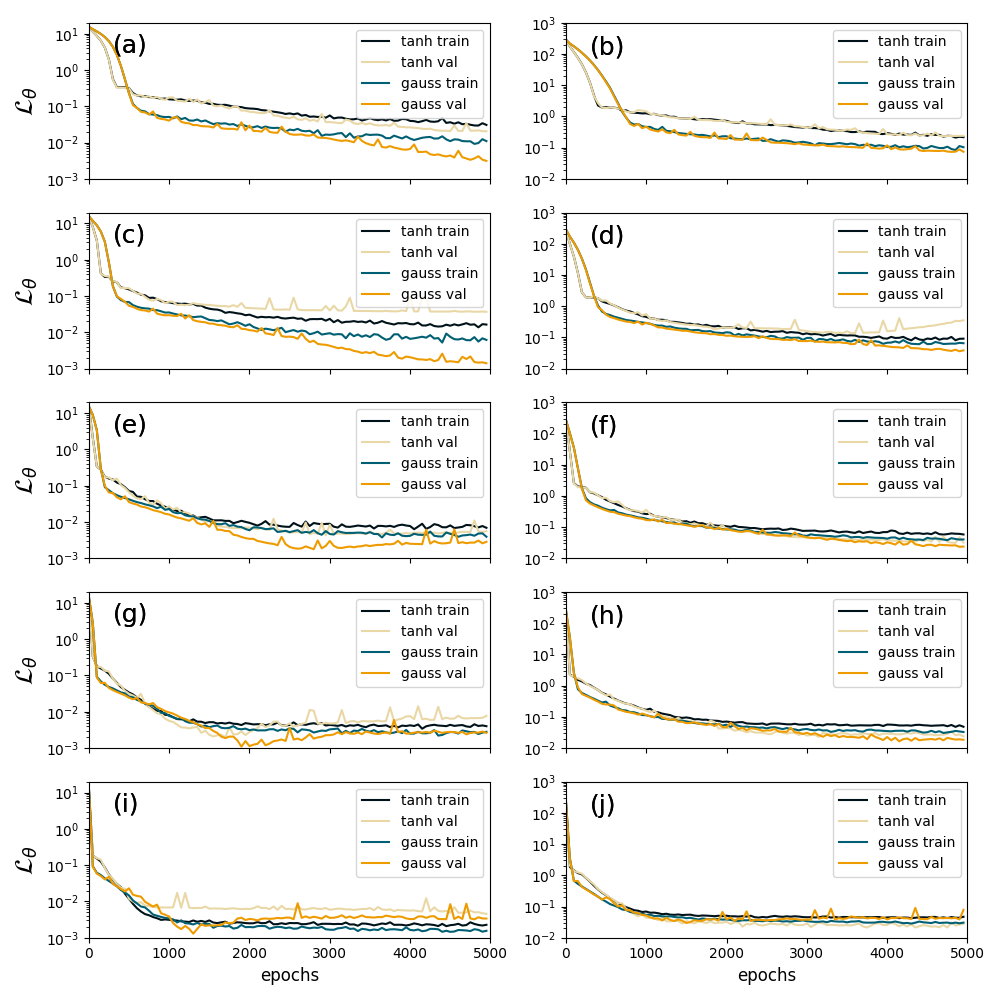
\includegraphics[width=0.8\textwidth]{./metrics_loss.png}
    \caption{Averaged in 5-folded loss functions calculated over 
    the training and the validation sets as function of the epoch. In all the cases 
    the number of layesrs $N_L = 2$. Left column: 
    $\mathcal{L}_\theta^{LCH}$ loss function, right column: 
    $\mathcal{L}_\theta^{ERR}$ loss function. Each row correspond 
    to architectures with increasing number of hidden units 
    $N_H = \left\{16, 32, 64, 128, 256, 512\right\}$, shown in
    panels (a) and (b); (c) and (d); (e) and (f); (g) and (h); 
    and (i) and (j), respectively.}
    \label{fig:training_losses}
\end{figure}

First, we want to point out that the increase of $N_L$ above two 
hidden layers does not produce significant improvements. A 
similar behavior occurs with the increasing of $N_H$ above 
$N_H =128$, as can be observed in Fig. \ref{fig:training_losses}. 
In this Figure we show the evolution of both
loss function during the hyperparamenter exploration process 
as function of the iteration number or \emph{epoch} of the 
optimization process. Moreover, we observe that 
$\mathcal{L}^{ERR}_{\theta}$ produces a smoother optimization 
curves, and, except for the case of $N_H=32$ with $\tanh$ 
activation function in panel (d) this loss does not produce 
overfitting or an increase in the loss during the optimization 
process. The opposite behavior can be observed for 
$\mathcal{L}^{LCH}_{\theta}$ in panels (c), (e) and (g). 
In the following, we use $\mathcal{L}^{ERR}_{\theta}$ 
as the loss function. We also observe that gaussian 
activation is more adequate. To examinate the behavior 
of the three terms of $\mathcal{L}^{ERR}_{\theta}$ 
we show in Fig. \ref{fig:main_metrics} the evolution during 
the training process for mean error functions over the validation 
set. The error computed are MAE (panels (a) and (b)), 
RMSE in panels (c) and (d), and MRE shown in panels (e) and (f).
The left column correspond to $\tan$ activation, meanwhile the 
right column to gaussian activation function respectively finding 
a behavior that confirms the use of $N_H=128$.
\begin{figure}[htbp]
    \centering
    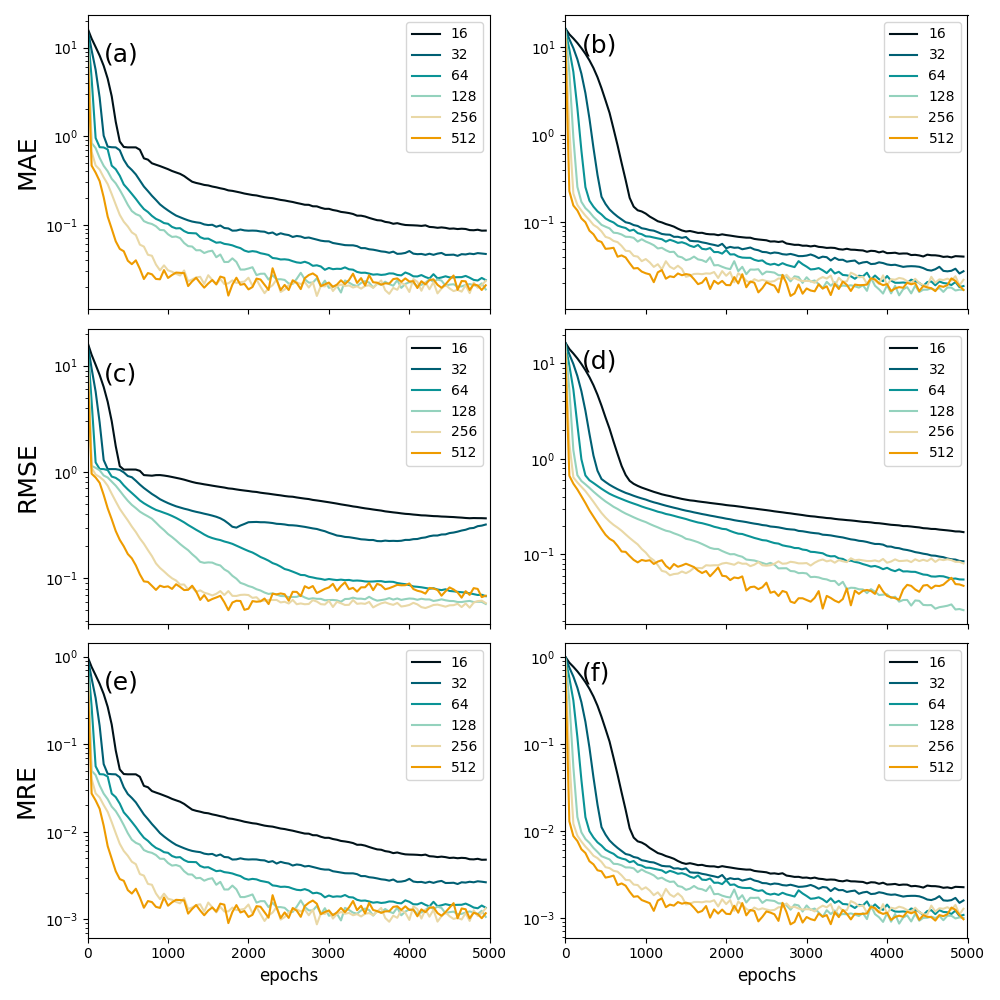
\includegraphics[width=0.8\textwidth]{./metrics_main.png}
    \caption{Metrics over validation set for different network 
    architectures. Left column (a, c, and e) metrics with $\tanh$ 
    activation function. Right column (b-d-f) gaussian activation 
    function. Each row correspond to a different metric over the 
    $\log_{10}$ of the TCS.}
    \label{fig:main_metrics}
\end{figure}


To get a deep understand of the activation function we explore 
the evolution of the maximum of the errors instead of mean values
in Fig. \ref{fig:max_metrics}. In this Figure we observe that 
gaussian activation exhibits monotonically decreasing errors 
for $N_H \le 128$ hidden units, in contrast to $\tanh$ activation 
which shows more erratic behavior. 

\begin{figure}[htbp]
    \centering
    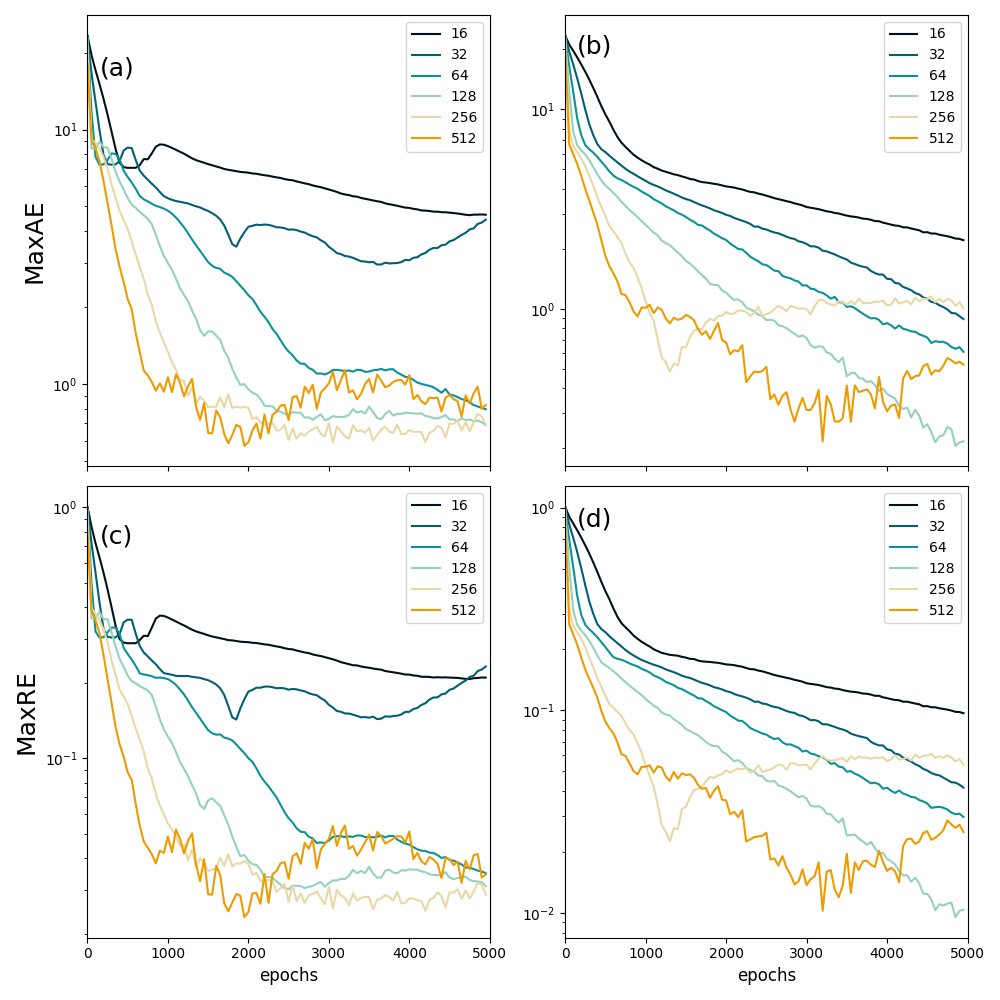
\includegraphics[width=0.8\textwidth]{./metrics_max.png}
    \caption{Maximum values of metrics over validation set 
    for different network architectures. 
    Left column (a, c) metrics with $\tanh$ 
    activation function. Right column (b-d) gaussian activation 
    function. Each row correspond to a different metric over the 
    $\log_{10}$ of the TCS.}
    \label{fig:max_metrics}
\end{figure}

With the above results we decide to use as the optimum model 
a MLP with two hidden layers with 128 units each, using a gaussian
activation function. This model has a total of 17409 trainable 
parameters.

\section{Results}
\label{sec:results}

In this work we fit total cross sections calculated by means of the 
CDW-EIS, CTMC, and the RSEM for ionization of hydrogen by bare 
projectiles with charges ranging from 1 to 9. 

This section can be divided in two main parts: one with the 
fits for the TCS for each case and the other with numerical 
experiments retraining models with missing data for particular 
projectile charges.


\subsection{Evaluation of the fits}

We perform evaluations over the whole TCS training set 
with the best model found in the previous section to understand 
the different errors in $cm^2$. It is important to note that 
we have interpolated the $\log_{10}(TCS)$, which leads to 
errors different to those shown in the previous section.

\begin{figure}[htbp]
    \centering
    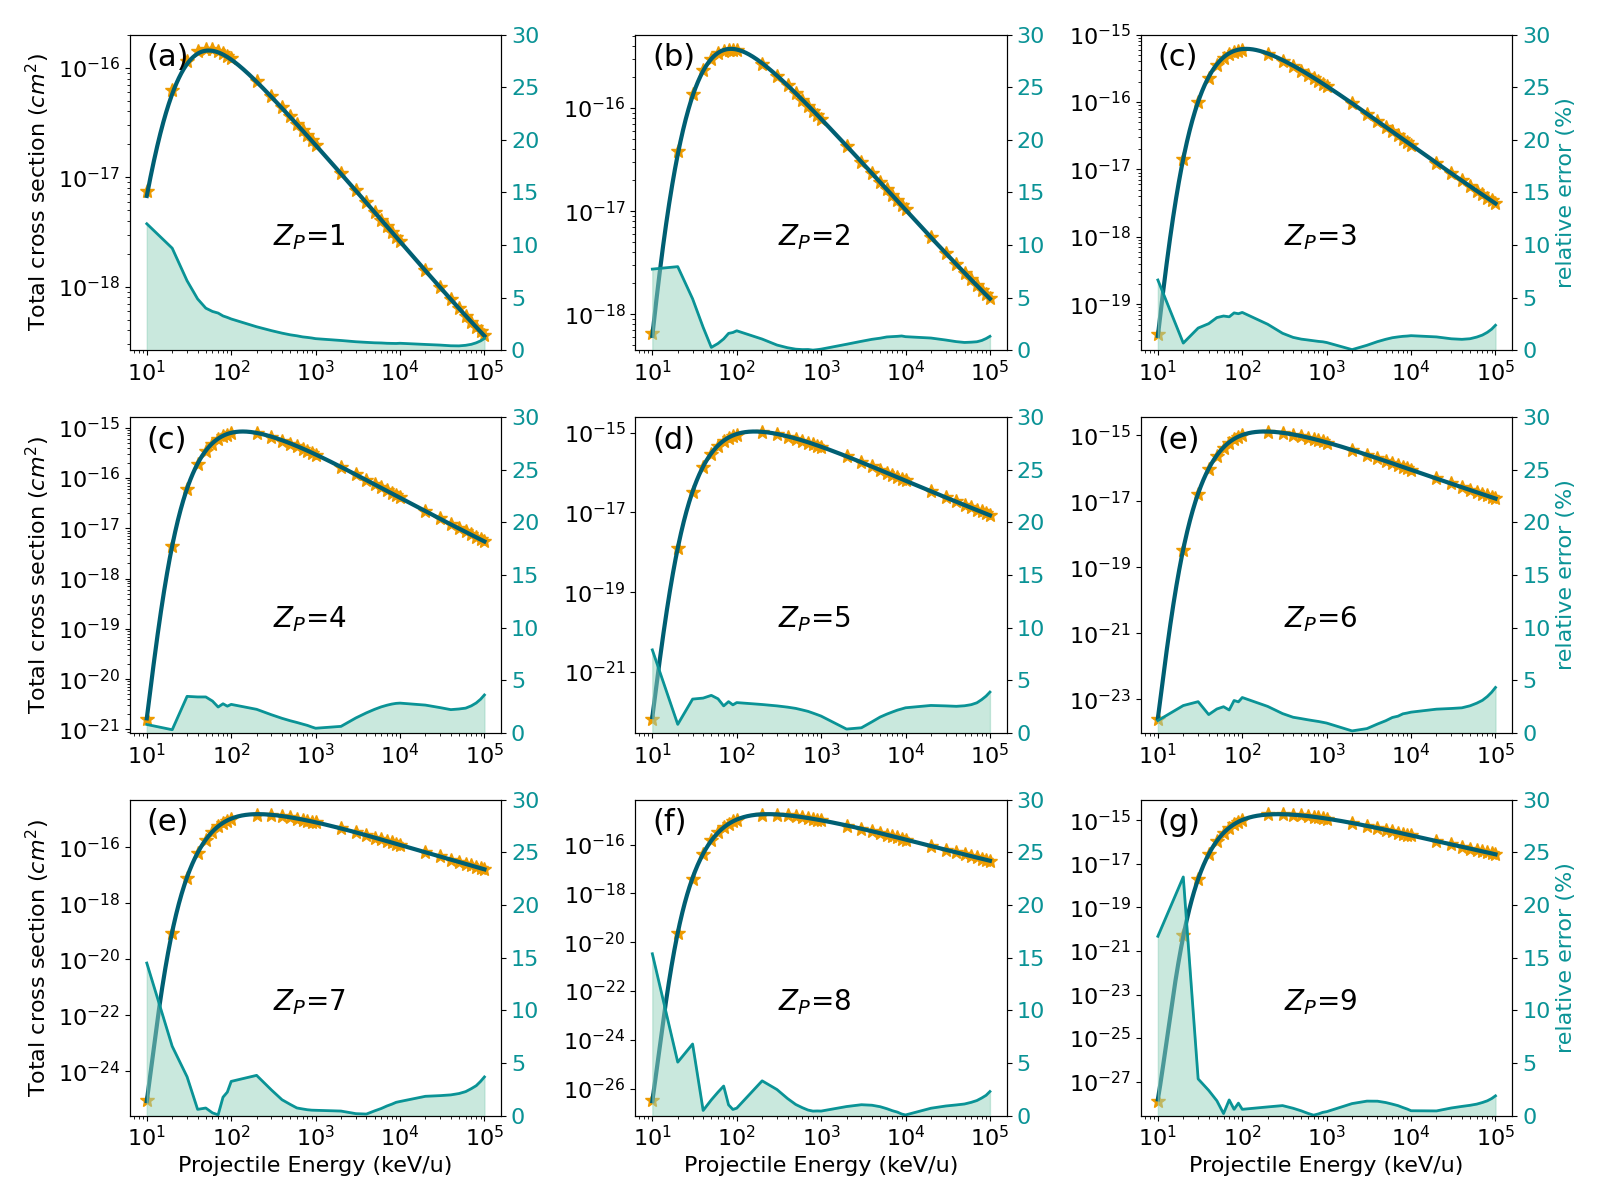
\includegraphics[width=0.8\textwidth]{./performance_CDWEIS.png}
    \caption{Solid lines: Prediction of the MLP for CDW-EIS calculations 
    as a function of the 
    projectile impact energy for different $Z_p$. Orange stars: calculated TCS. 
    Panels (a) to (g) correspond to $ Z_P=1$ to $Z_P = 9$ respectively. 
    Relative error is drawn as green filled curve. The right 
    axis scale correspond to the percentage relative error calculated at the 
    ground truth values of the TCS.}
    \label{fig:performance_cdweis}
\end{figure}

\begin{figure}[htbp]
    \centering
    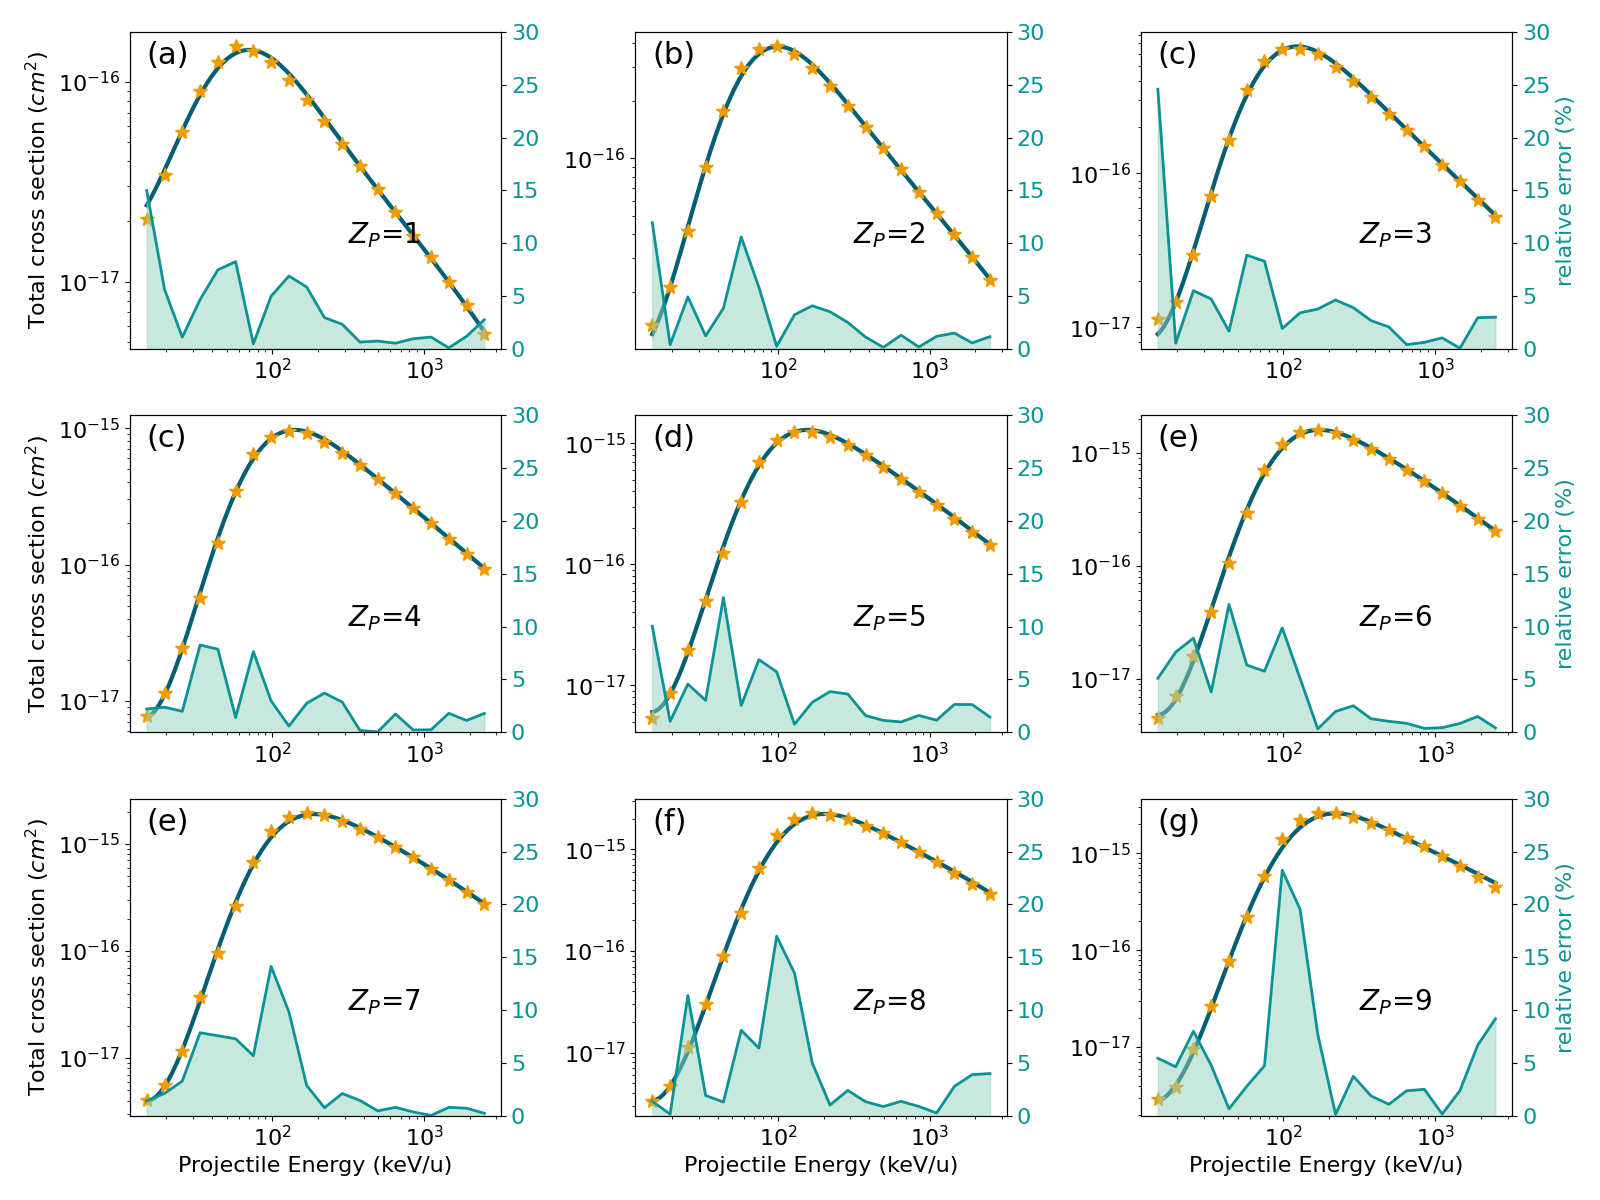
\includegraphics[width=0.8\textwidth]{./performance_CTMC.png}
    \caption{Prediction of the MLP and percentage relative 
    errors as in Fig. \ref{fig:performance_cdweis} for CTMC calculations 
    as a function of the 
    projectile impact energy for different $Z_p$. }
    \label{fig:performance_ctmc}
\end{figure}

\begin{figure}[htbp]
    \centering
    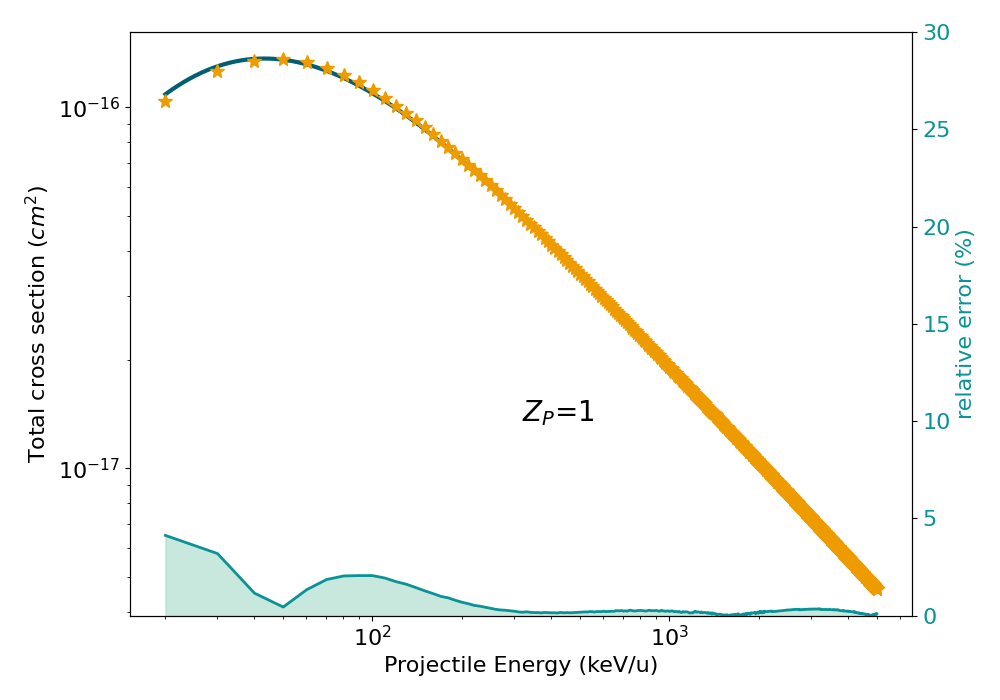
\includegraphics[width=0.8\textwidth]{./performance_RSEM.png}
    \caption{Prediction of the MLP and percentage relative 
    errors as in Fig. \ref{fig:performance_cdweis} for RSEM calculations 
    as a function of the 
    projectile impact energy for $Z_p = 1$. }
    \label{fig:performance_rsem}
\end{figure}

We show in Figures \ref{fig:performance_cdweis} and \ref{fig:performance_ctmc} 
the performance for MLP to fit the calculated data. We observe 
relative errors below five percent for high energies where the 
cross sections present smooth changes. In the low energy region 
where TCS changes several orders of magnitude the error raises up to 
15\%. In the case of RSEM fitting, the error is under 3\%. The main reason of 
this accuracy is directly related to the number of TCS calculated for training.
At this point, it is very important to recall that MLP is a single regressor for 
the three models and the 9 projectile charges considered here, i.e. all the 
curves are reproduced with the same fitting model.

\subsection{Interpolation and extrapolation}

To address the power of the MLP as interpolator, we perform a fitting 
process excluding the data of TCS calculated for $Z_P=3$. The architecture 
of the MLP (the hypeperparameters) remains untouched respect to the full 
training set. We perform a splitting for validation as in the former case, 
and explore the ability to interpolate over the unseen by the model data.

\begin{figure}[htbp]
    \centering
    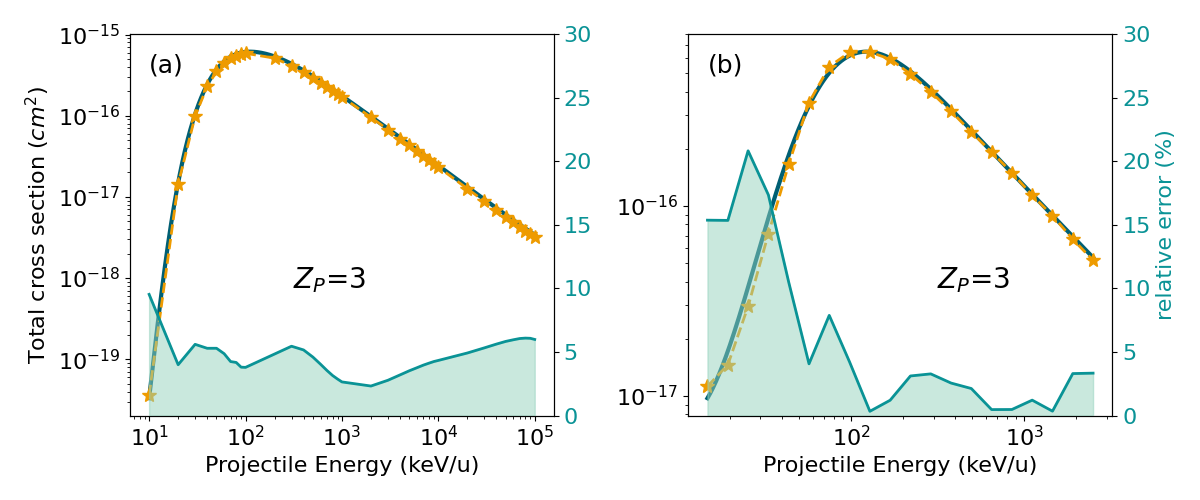
\includegraphics[width=0.8\textwidth]{./performance_gausshole_3.png}
    \caption{Prediction of the MLP and percentage relative 
    errors as in Fig. \ref{fig:performance_cdweis} for TCS calculated within 
    CDWEIS (panel(a)) and CTMC (panel(b)) as a function of the 
    projectile impact energy for $Z_p = 3$. Stars: calculations, 
    solid lines: MLP interpolation.}
    \label{fig:performance_interpolation_3}
\end{figure}


We show in the Figure \ref{fig:performance_interpolation_3} the results 
compared to the calculated cross sections as function of the projectile  
impact energy. We observe a remarkable behavior of the model to 
interpolate TCS for two theories and a wide range of energies in the 
$Z_P$ axis. Naturally, as it was observed in the former fitting case of 
this dataset, the MLP present higher percentage relative errors for low 
impact energies where the TCS vary several orders of magnitude.

To explore the extrapolation case, we perform a similar analysis excluding 
the case of $Z_P=9$, this means that we push the model to extrapolate TCS 
for the whole energy range and the two thoretical models.
We show in Fig. \ref{fig:performance_extrapolation_9} results for 
extrapolation case. Results are not as good as in the case 
of interpolation, but naturally, the predictions are smooth, since 
gaussian activations are used, and relative errors does not exceed 35\% 
in the whole impact energy range considered, except for the case of CDW-EIS at 
$E_P = 10 keV/u$

\begin{figure}[htbp]
    \centering
    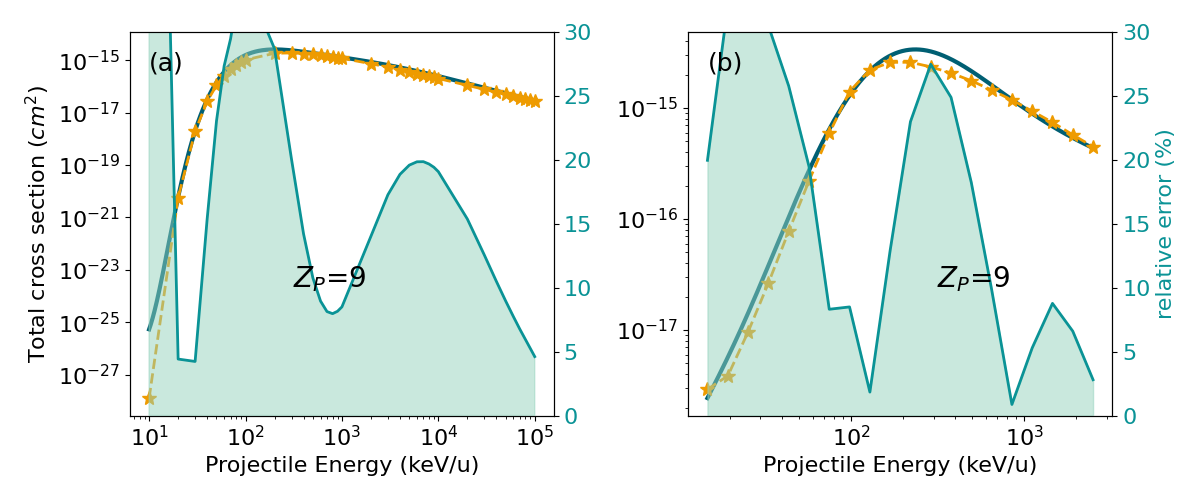
\includegraphics[width=0.8\textwidth]{./performance_gausshole_9.png}
    \caption{Prediction of the MLP and percentage relative 
    errors as in Fig. \ref{fig:performance_cdweis} for TCS calculated within 
    CDWEIS (panel(a)) and CTMC (panel(b)) as a function of the 
    projectile impact energy for $Z_p = 9$. Stars: calculations, 
    solid lines: MLP extrapolation.}
    \label{fig:performance_extrapolation_9}
\end{figure}


% \begin{table}[h]
%     \centering
%     \begin{tabular}{|l|cc|cc|cc|cc|}
%         \hline
%         \textbf{Hole} & \multicolumn{2}{c|}{\textbf{MAE}} & \multicolumn{2}{c|}{\textbf{MRE}} & \multicolumn{2}{c|}{\textbf{MAX MAE}} & \multicolumn{2}{c|}{\textbf{MAX MRE}} \\ \cline{2-9} 
%                       & All & Holes & All & Holes & All & Holes & All & Holes \\ \hline 
%         3             &     &       &     &       &     &       &     &       \\
%         3,4           &     &       &     &       &     &       &     &       \\ \hline
%     \end{tabular}
% \end{table}

\section{Discussion}
\label{sec:discussion}


\section{Conclusion}
\label{sec:conclusion}

Summarize your conclusions and future work.

\begin{thebibliography}{99}

\bibitem{ref1} Author, ``Title,'' \textit{Journal}, vol. X, pp. XX-XX, Year.

\end{thebibliography}

\end{document}